% mnras_template.tex
%
% LaTeX template for creating an MNRAS paper
%
% v3.0 released 14 May 2015
% (version numbers match those of mnras.cls)
%
% Copyright (C) Royal Astronomical Society 2015
% Authors:
% Keith T. Smith (Royal Astronomical Society)

% Change log
%
% v3.0 May 2015
%    Renamed to match the new package name
%    Version number matches mnras.cls
%    A few minor tweaks to wording
% v1.0 September 2013
%    Beta testing only - never publicly released
%    First version: a simple (ish) template for creating an MNRAS paper

%%%%%%%%%%%%%%%%%%%%%%%%%%%%%%%%%%%%%%%%%%%%%%%%%%
% Basic setup. Most papers should leave these options alone.
\documentclass[fleqn,usenatbib]{mnras}  % a4paper,

% MNRAS is set in Times font. If you don't have this installed (most LaTeX
% installations will be fine) or prefer the old Computer Modern fonts, comment
% out the following line
%\usepackage{newtxtext,newtxmath}
%\usepackage{lmodern}
% Depending on your LaTeX fonts installation, you might get better results with one of these:
\usepackage{mathptmx}
%\usepackage{txfonts}


% Use vector fonts, so it zooms properly in on-screen viewing software
% Don't change these lines unless you know what you are doing
\usepackage[T1]{fontenc}
\usepackage{ae,aecompl}
\usepackage{slashbox}

%%%%% AUTHORS - PLACE YOUR OWN PACKAGES HERE %%%%%

% Only include extra packages if you really need them. Common packages are:
\usepackage{graphicx}	% Including figure files
\usepackage{amsmath}	% Advanced maths commands
\usepackage{amssymb}	% Extra maths symbols
\usepackage{savesym}  % prevent symbol conflicts
\savesymbol{sf}
%\generate{%
%  \file{breqn.sty}{\nopreamble\from{breqn.dtx}{breqn.sty}}%
%}
%\usepackage{breqn} % automatic breaking equation 
%\usepackage{fancyvrb}
%\VerbatimFootnotes
\usepackage{cprotect}  % to allow verb in caption 
\DeclareMathOperator\erfc{erfc}
\DeclareMathOperator\erf{erf}
\DeclareMathOperator\cdf{cdf}
\DeclareMathOperator\sf{sf}
\DeclareMathOperator\isf{isf}
\DeclareMathOperator\ppf{ppf}

%%%%%%%%%%%%%%%%%%%%%%%%%%%%%%%%%%%%%%%%%%%%%%%%%%

%%%%% AUTHORS - PLACE YOUR OWN COMMANDS HERE %%%%%

% Please keep new commands to a minimum, and use \newcommand not \def to avoid
% overwriting existing commands. Example:
%\newcommand{\pcm}{\,cm$^{-2}$}	% per cm-squared

%%%%%%%%%%%%%%%%%%%%%%%%%%%%%%%%%%%%%%%%%%%%%%%%%%

%%%%%%%%%%%%%%%%%%% TITLE PAGE %%%%%%%%%%%%%%%%%%%

% Title of the paper, and the short title which is used in the headers.
% Keep the title short and informative.
\title[SDSS Quasars]{SDSS Stripe 82 : quasar variability from forced photometry}

% The list of authors, and the short list which is used in the headers.
% If you need two or more lines of authors, add an extra line using \newauthor
\author[K. Suberlak et al.]{
Krzysztof Suberlak,$^{1}$\thanks{E-mail: suberlak@uw.edu}
\v{Z}eljko Ivezi\'c, $^{1}$
Yusra AlSayyad,$^{1}$ 
\\
% List of institutions
$^{1}$Department of Astronomy, University of Washington, Seattle, WA, United States\\
}

% These dates will be filled out by the publisher
\date{Accepted XXX. Received YYY; in original form ZZZ}

% Enter the current year, for the copyright statements etc.
\pubyear{2015}

% Don't change these lines
\begin{document}
\label{firstpage}
\pagerange{\pageref{firstpage}--\pageref{lastpage}}
\maketitle

% Abstract of the paper
\begin{abstract}

\end{abstract}


%%%%%%%%%%%%%%%%%%%%%%%%%%%%%%%%%%%%%%%%%%%%%%%%%%

%%%%%%%%%%%%%%%%% BODY OF PAPER %%%%%%%%%%%%%%%%%%



\section{Variability}

Many lightcurves display an intrinsic variability, in addition to the  error-induced noise. A lightcurve consists of a set of N measurements and associated errors {$x_{i}, e_{i}$} of the object brightness. In this analysis we assume that  $x_{i}$ are drawn from a Gaussian distribution  $\mathcal{N}(\mu,\sigma)$, and that errors $e_{i}$ are homoscedastic, so that  the distribution of measurements is Gaussian.  In this framework $\mu$ describes the median value of brightness, which for non-variable objects is the true brightness.  Using the Bayesian approach, to find $\mu$  we seek to maximize the posterior probability distribution function (pdf) of  $\mu$ given $x_{i}$ and $e_{i}$ : $p(\mu | {x_{i}},{\sigma_{i}})$.  We can proceed analoguously to find the width of the distribution, $\sigma$, which describes the  departure from the mean. 

To find $\mu$ and $\sigma$, we follow Ivezic+2014, with the two-step approach:  first we find approximate values of  $\mu_{0}$ and $\sigma_{0}$, and then we evaluate the full logarithm of the posterior pdf in the vicinity of the approximate solution. The maximum of the 2D likelihood becomes our full solution - $\sigma_{full}$ and $\mu_{full}$ (see Appendix B for the detailed calculation). 

For each lightcurve, we also calculate mean-based $\chi^{2}_{DOF}$ and median-based $\chi^{2}_{R}$ (the latter is more robust against any outliers in the distribution) : 

\begin{equation}
\label{eqn:chi2DOF}
\chi^{2}_{dof} = \frac{1}{N-1}\sum{\left( \frac{x_{i} - <x_{i}>} {e_{i}} \right) ^{2}}
\end{equation}

and 
\begin{equation}
\label{eqn:chi2R}
\chi^{2}_{R} = 0.7414 (Z_{75\%} - Z_{25\%} ) 
\end{equation}

with $Z=(x_{i} - median(x_{i})) / e_{i} $. 

Initially, we evaluate $\mu_{full}$, $\sigma_{full}$, $\chi^{2}_{dof}$, and $\chi^{2}_{R}$ for the entire lightcurve. Then, only if  either $\sigma_{full}>0$ or $\chi^{2}>1 $, which hints some intrinsic variability, we also calculate $mu_{full}$, $\sigma_{full}$, and $\chi^{2}$ for the seasonally-binned portions of the lightcurve.   


\begin{figure*}
\label{fig:sigma_example}
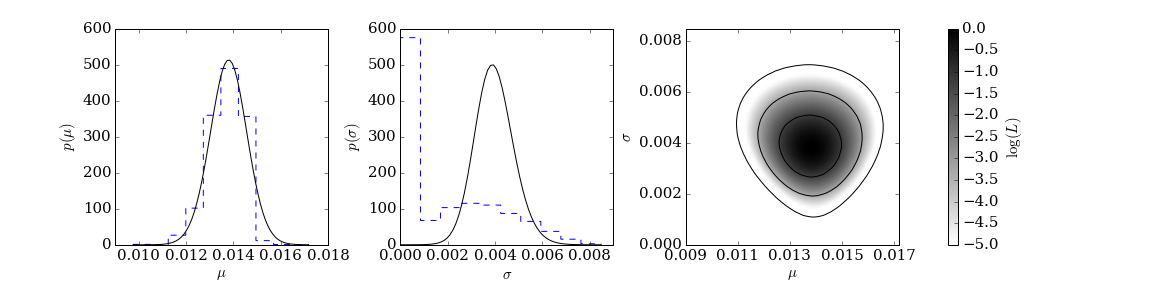
\includegraphics[width=\textwidth]{Fig_5-8_AstroML_obj_217720894888346446_.png}
\cprotect\caption{Two-step approach to finding $\mu$ and $\sigma$ via $\mu_{0}$ and $\sigma_{0}$ for an object 217720894888346446. In this calculation we use raw psf flux, before employing the faint source treatment outlined in Section~\ref{sec:faint_sources}. On the left and middle panels,  solid lines trace marginalized posterior pdfs for $\mu$ and $\sigma$ , while dashed lines depict histogram distributions of 10,000 bootstrap resamples for $\mu_{0}$ and $\sigma_{0}$. The right panel shows the logarithm of the posterior probability density function for $\mu$ and $\sigma$.}
\end{figure*}

%%%%%%%%%%%%%%%%%%%%%%%%%%%%%%%%%%%%%%%%%%%%%%%%%%

%%%%%%%%%%%%%%%%%%%% REFERENCES %%%%%%%%%%%%%%%%%%

% The best way to enter references is to use BibTeX:

%\bibliographystyle{mnras}
%\bibliography{example} % if your bibtex file is called example.bib

%%%%%%%%%%%%%%%%%%%%%%%%%%%%%%%%%%%%%%%%%%%%%%%%%%


% Don't change these lines
\bsp	% typesetting comment
\label{lastpage}
\end{document}

% End of mnras_template.tex
